%%%%%%%%%%%%%%%%%%%%%%%%%%%%%%%%%%%%%%%%%
% Lachaise Assignment
% LaTeX Template
% Version 1.0 (26/6/2018)
%
% This template originates from:
% http://www.LaTeXTemplates.com
%
% Authors:
% Marion Lachaise & François Févotte
% Vel (vel@LaTeXTemplates.com)
%
% License:
% CC BY-NC-SA 3.0 (http://creativecommons.org/licenses/by-nc-sa/3.0/)
% 
%%%%%%%%%%%%%%%%%%%%%%%%%%%%%%%%%%%%%%%%%

%----------------------------------------------------------------------------------------
%	PACKAGES AND OTHER DOCUMENT CONFIGURATIONS
%----------------------------------------------------------------------------------------

\documentclass{article}

%%%%%%%%%%%%%%%%%%%%%%%%%%%%%%%%%%%%%%%%%
% Lachaise Assignment
% Structure Specification File
% Version 1.0 (26/6/2018)
%
% This template originates from:
% http://www.LaTeXTemplates.com
%
% Authors:
% Marion Lachaise & François Févotte
% Vel (vel@LaTeXTemplates.com)
%
% License:
% CC BY-NC-SA 3.0 (http://creativecommons.org/licenses/by-nc-sa/3.0/)
% 
%%%%%%%%%%%%%%%%%%%%%%%%%%%%%%%%%%%%%%%%%

%----------------------------------------------------------------------------------------
%	PACKAGES AND OTHER DOCUMENT CONFIGURATIONS
%----------------------------------------------------------------------------------------

\usepackage{luacode}

\usetikzlibrary{positioning}

\usepackage{mathtools}
\usepackage{slashed}
\usepackage{pgfplots}
\pgfplotsset{compat=1.7}
\usepackage{float}
\usepackage{ulem}


\usepackage{amsmath,amsfonts,stmaryrd,amssymb} % Math packages

\usepackage{enumerate} % Custom item numbers for enumerations

\usepackage[ruled]{algorithm2e} % Algorithms

\usepackage[framemethod=tikz]{mdframed} % Allows defining custom boxed/framed environments

\usepackage{listings} % File listings, with syntax highlighting
\lstset{
	basicstyle=\ttfamily, % Typeset listings in monospace font
}

%----------------------------------------------------------------------------------------
%	DOCUMENT MARGINS
%----------------------------------------------------------------------------------------

\usepackage{geometry} % Required for adjusting page dimensions and margins

\geometry{
	paper=a4paper, % Paper size, change to letterpaper for US letter size
	top=2.5cm, % Top margin
	bottom=3cm, % Bottom margin
	left=2.5cm, % Left margin
	right=2.5cm, % Right margin
	headheight=14pt, % Header height
	footskip=1.5cm, % Space from the bottom margin to the baseline of the footer
	headsep=1.2cm, % Space from the top margin to the baseline of the header
	%showframe, % Uncomment to show how the type block is set on the page
}

%----------------------------------------------------------------------------------------
%	FONTS
%----------------------------------------------------------------------------------------

\usepackage[utf8]{inputenc} % Required for inputting international characters
\usepackage[T1]{fontenc} % Output font encoding for international characters

\usepackage{XCharter} % Use the XCharter fonts


% MY SHIT
%--------------------------------
\def\doubleunderline#1{\underline{\underline{#1}}}
\usepackage{xparse}

\NewDocumentCommand{\INTERVALINNARDS}{ m m }{
	#1 {,} #2
}
\NewDocumentCommand{\interval}{ s m >{\SplitArgument{1}{,}}m m o }{
	\IfBooleanTF{#1}{
		\left#2 \INTERVALINNARDS #3 \right#4
	}{
		\IfValueTF{#5}{
			#5{#2} \INTERVALINNARDS #3 #5{#4}
		}{
			#2 \INTERVALINNARDS #3 #4
		}
	}
}


\newcommand\neginfinf{\stackrel{\mathclap{\normalfont\mbox{$\left[\frac{-\infty}{\infty}\right]$}}}{=}}
\newcommand\infinf{\stackrel{\mathclap{\normalfont\mbox{$\left[\frac{\infty}{\infty}\right]$}}}{=}}
\newcommand\nillnill{\stackrel{\mathclap{\normalfont\mbox{$\left[\frac{0}{0}\right]$}}}{=}}

\newcommand*{\skippingparagraph}{\par\vspace{\baselineskip}\noindent}


%------------------------------------




%----------------------------------------------------------------------------------------
%	COMMAND LINE ENVIRONMENT
%----------------------------------------------------------------------------------------

% Usage:
% \begin{commandline}
%	\begin{verbatim}
%		$ ls
%		
%		Applications	Desktop	...
%	\end{verbatim}
% \end{commandline}

\mdfdefinestyle{commandline}{
	leftmargin=10pt,
	rightmargin=10pt,
	innerleftmargin=15pt,
	middlelinecolor=black!50!white,
	middlelinewidth=2pt,
	frametitlerule=false,
	backgroundcolor=black!5!white,
	frametitle={Command Line},
	frametitlefont={\normalfont\sffamily\color{white}\hspace{-1em}},
	frametitlebackgroundcolor=black!50!white,
	nobreak,
}

% Define a custom environment for command-line snapshots
\newenvironment{commandline}{
	\medskip
	\begin{mdframed}[style=commandline]
}{
	\end{mdframed}
	\medskip
}

%----------------------------------------------------------------------------------------
%	FILE CONTENTS ENVIRONMENT
%----------------------------------------------------------------------------------------

% Usage:
% \begin{file}[optional filename, defaults to "File"]
%	File contents, for example, with a listings environment
% \end{file}

\mdfdefinestyle{file}{
	innertopmargin=1.6\baselineskip,
	innerbottommargin=0.8\baselineskip,
	topline=false, bottomline=false,
	leftline=false, rightline=false,
	leftmargin=2cm,
	rightmargin=2cm,
	singleextra={%
		\draw[fill=black!10!white](P)++(0,-1.2em)rectangle(P-|O);
		\node[anchor=north west]
		at(P-|O){\ttfamily\mdfilename};
		%
		\def\l{3em}
		\draw(O-|P)++(-\l,0)--++(\l,\l)--(P)--(P-|O)--(O)--cycle;
		\draw(O-|P)++(-\l,0)--++(0,\l)--++(\l,0);
	},
	nobreak,
}

% Define a custom environment for file contents
\newenvironment{file}[1][File]{ % Set the default filename to "File"
	\medskip
	\newcommand{\mdfilename}{#1}
	\begin{mdframed}[style=file]
}{
	\end{mdframed}
	\medskip
}

%----------------------------------------------------------------------------------------
%	NUMBERED QUESTIONS ENVIRONMENT
%----------------------------------------------------------------------------------------

% Usage:
% \begin{question}[optional title]
%	Question contents
% \end{question}

\mdfdefinestyle{question}{
	innertopmargin=1.2\baselineskip,
	innerbottommargin=0.8\baselineskip,
	roundcorner=5pt,
	nobreak,
	singleextra={%
		\draw(P-|O)node[xshift=1em,anchor=west,fill=white,draw,rounded corners=5pt]{%
		Question \theQuestion\questionTitle};
	},
}

\newcounter{Question} % Stores the current question number that gets iterated with each new question

% Define a custom environment for numbered questions
\newenvironment{question}[1][\unskip]{
	\bigskip
	\stepcounter{Question}
	\newcommand{\questionTitle}{~#1}
	\begin{mdframed}[style=question]
}{
	\end{mdframed}
	\medskip
}

%----------------------------------------------------------------------------------------
%	WARNING TEXT ENVIRONMENT
%----------------------------------------------------------------------------------------

% Usage:
% \begin{warn}[optional title, defaults to "Warning:"]
%	Contents
% \end{warn}

\mdfdefinestyle{warning}{
	topline=false, bottomline=false,
	leftline=false, rightline=false,
	nobreak,
	singleextra={%
		\draw(P-|O)++(-0.5em,0)node(tmp1){};
		\draw(P-|O)++(0.5em,0)node(tmp2){};
		\fill[black,rotate around={45:(P-|O)}](tmp1)rectangle(tmp2);
		\node at(P-|O){\color{white}\scriptsize\bf !};
		\draw[very thick](P-|O)++(0,-1em)--(O);%--(O-|P);
	}
}

% Define a custom environment for warning text
\newenvironment{warn}[1][Warning:]{ % Set the default warning to "Warning:"
	\medskip
	\begin{mdframed}[style=warning]
		\noindent{\textbf{#1}}
}{
	\end{mdframed}
}

%----------------------------------------------------------------------------------------
%	INFORMATION ENVIRONMENT
%----------------------------------------------------------------------------------------

% Usage:
% \begin{info}[optional title, defaults to "Info:"]
% 	contents
% 	\end{info}

\mdfdefinestyle{info}{%
	topline=false, bottomline=false,
	leftline=false, rightline=false,
	nobreak,
	singleextra={%
		\fill[black](P-|O)circle[radius=0.4em];
		\node at(P-|O){\color{white}\scriptsize\bf i};
		\draw[very thick](P-|O)++(0,-0.8em)--(O);%--(O-|P);
	}
}

% Define a custom environment for information
\newenvironment{info}[1][Info:]{ % Set the default title to "Info:"
	\medskip
	\begin{mdframed}[style=info]
		\noindent{\textbf{#1}}
}{
	\end{mdframed}
}
 % Include the file specifying the document structure and custom commands

%----------------------------------------------------------------------------------------
%	ASSIGNMENT INFORMATION
%----------------------------------------------------------------------------------------

\title{MAT-1001: Obligatorisk oppgave} % Title of the assignment

\author{Theodor Tollersrud\\ \texttt{tto061@uit.no}} % Author name and email address

\date{Universitetet i Tromsø --- \today} % University, school and/or department name(s) and a date

%----------------------------------------------------------------------------------------

\begin{document}

\maketitle % Print the title

%----------------------------------------------------------------------------------------
%	INTRODUCTION
%----------------------------------------------------------------------------------------
$$\bigoplus_{i=0}^{m} x_i$$
$$\bigparallel_{i=0}^{m} x_i$$

\section*{Oppgave 1} % Unnumbered section
\subsection*{a)}
\begin{align*}
	z^2 - az + 1 = 0\\
	z = \frac{a \pm \sqrt{a^2 - 4}}{2}
\end{align*}
\begin{figure}[H]
	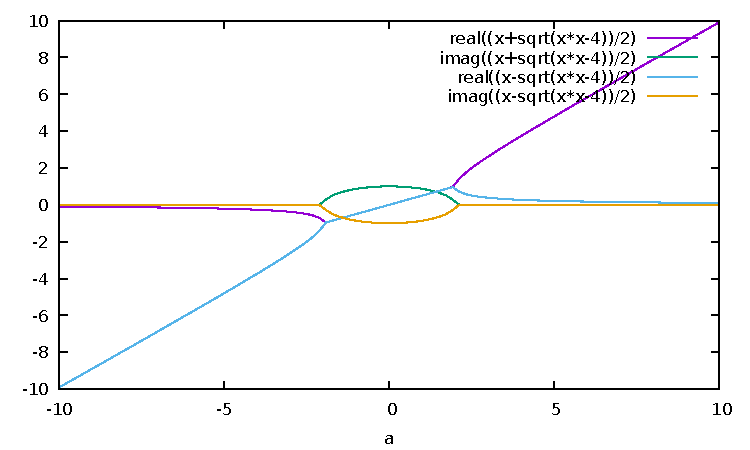
\includegraphics[width=\textwidth]{output.pdf}
\end{figure}
I intervallet $\interval({2, 2})$ har ligningen komplekse løsninger. Utenfor dette intervallet er den komplekse delen av løsningene 0. 

% GNUPLOT: LaTeX picture with Postscript
\begingroup
  \makeatletter
  \providecommand\color[2][]{%
    \GenericError{(gnuplot) \space\space\space\@spaces}{%
      Package color not loaded in conjunction with
      terminal option `colourtext'%
    }{See the gnuplot documentation for explanation.%
    }{Either use 'blacktext' in gnuplot or load the package
      color.sty in LaTeX.}%
    \renewcommand\color[2][]{}%
  }%
  \providecommand\includegraphics[2][]{%
    \GenericError{(gnuplot) \space\space\space\@spaces}{%
      Package graphicx or graphics not loaded%
    }{See the gnuplot documentation for explanation.%
    }{The gnuplot epslatex terminal needs graphicx.sty or graphics.sty.}%
    \renewcommand\includegraphics[2][]{}%
  }%
  \providecommand\rotatebox[2]{#2}%
  \@ifundefined{ifGPcolor}{%
    \newif\ifGPcolor
    \GPcolortrue
  }{}%
  \@ifundefined{ifGPblacktext}{%
    \newif\ifGPblacktext
    \GPblacktexttrue
  }{}%
  % define a \g@addto@macro without @ in the name:
  \let\gplgaddtomacro\g@addto@macro
  % define empty templates for all commands taking text:
  \gdef\gplbacktext{}%
  \gdef\gplfronttext{}%
  \makeatother
  \ifGPblacktext
    % no textcolor at all
    \def\colorrgb#1{}%
    \def\colorgray#1{}%
  \else
    % gray or color?
    \ifGPcolor
      \def\colorrgb#1{\color[rgb]{#1}}%
      \def\colorgray#1{\color[gray]{#1}}%
      \expandafter\def\csname LTw\endcsname{\color{white}}%
      \expandafter\def\csname LTb\endcsname{\color{black}}%
      \expandafter\def\csname LTa\endcsname{\color{black}}%
      \expandafter\def\csname LT0\endcsname{\color[rgb]{1,0,0}}%
      \expandafter\def\csname LT1\endcsname{\color[rgb]{0,1,0}}%
      \expandafter\def\csname LT2\endcsname{\color[rgb]{0,0,1}}%
      \expandafter\def\csname LT3\endcsname{\color[rgb]{1,0,1}}%
      \expandafter\def\csname LT4\endcsname{\color[rgb]{0,1,1}}%
      \expandafter\def\csname LT5\endcsname{\color[rgb]{1,1,0}}%
      \expandafter\def\csname LT6\endcsname{\color[rgb]{0,0,0}}%
      \expandafter\def\csname LT7\endcsname{\color[rgb]{1,0.3,0}}%
      \expandafter\def\csname LT8\endcsname{\color[rgb]{0.5,0.5,0.5}}%
    \else
      % gray
      \def\colorrgb#1{\color{black}}%
      \def\colorgray#1{\color[gray]{#1}}%
      \expandafter\def\csname LTw\endcsname{\color{white}}%
      \expandafter\def\csname LTb\endcsname{\color{black}}%
      \expandafter\def\csname LTa\endcsname{\color{black}}%
      \expandafter\def\csname LT0\endcsname{\color{black}}%
      \expandafter\def\csname LT1\endcsname{\color{black}}%
      \expandafter\def\csname LT2\endcsname{\color{black}}%
      \expandafter\def\csname LT3\endcsname{\color{black}}%
      \expandafter\def\csname LT4\endcsname{\color{black}}%
      \expandafter\def\csname LT5\endcsname{\color{black}}%
      \expandafter\def\csname LT6\endcsname{\color{black}}%
      \expandafter\def\csname LT7\endcsname{\color{black}}%
      \expandafter\def\csname LT8\endcsname{\color{black}}%
    \fi
  \fi
    \setlength{\unitlength}{0.0500bp}%
    \ifx\gptboxheight\undefined%
      \newlength{\gptboxheight}%
      \newlength{\gptboxwidth}%
      \newsavebox{\gptboxtext}%
    \fi%
    \setlength{\fboxrule}{0.5pt}%
    \setlength{\fboxsep}{1pt}%
\begin{picture}(7200.00,5040.00)%
    \gplgaddtomacro\gplbacktext{%
      \csname LTb\endcsname%%
      \put(901,1592){\makebox(0,0){\strut{}$-3$}}%
      \put(1412,1406){\makebox(0,0){\strut{}$-2$}}%
      \put(1922,1220){\makebox(0,0){\strut{}$-1$}}%
      \put(2433,1034){\makebox(0,0){\strut{}$0$}}%
      \put(2944,848){\makebox(0,0){\strut{}$1$}}%
      \put(3454,662){\makebox(0,0){\strut{}$2$}}%
      \put(3964,476){\makebox(0,0){\strut{}$3$}}%
      \put(4194,511){\makebox(0,0)[l]{\strut{}$-3$}}%
      \put(4552,777){\makebox(0,0)[l]{\strut{}$-2$}}%
      \put(4909,1043){\makebox(0,0)[l]{\strut{}$-1$}}%
      \put(5267,1309){\makebox(0,0)[l]{\strut{}$0$}}%
      \put(5625,1574){\makebox(0,0)[l]{\strut{}$1$}}%
      \put(5982,1840){\makebox(0,0)[l]{\strut{}$2$}}%
      \put(6340,2106){\makebox(0,0)[l]{\strut{}$3$}}%
      \put(870,1710){\makebox(0,0)[r]{\strut{}$-3$}}%
      \put(870,1937){\makebox(0,0)[r]{\strut{}$-2$}}%
      \put(870,2164){\makebox(0,0)[r]{\strut{}$-1$}}%
      \put(870,2392){\makebox(0,0)[r]{\strut{}$0$}}%
      \put(870,2619){\makebox(0,0)[r]{\strut{}$1$}}%
      \put(870,2845){\makebox(0,0)[r]{\strut{}$2$}}%
      \put(870,3072){\makebox(0,0)[r]{\strut{}$3$}}%
    }%
    \gplgaddtomacro\gplfronttext{%
      \csname LTb\endcsname%%
      \put(5955,4536){\makebox(0,0)[r]{\strut{}$\frac{a - \sqrt{4a^2 - 4}}{2}$}}%
      \csname LTb\endcsname%%
      \put(5955,4316){\makebox(0,0)[r]{\strut{}$\frac{a + \sqrt{4a^2 - 4}}{2}$}}%
      \csname LTb\endcsname%%
      \put(2075,815){\makebox(0,0){\strut{}a}}%
      \put(5779,1155){\makebox(0,0){\strut{}imag}}%
      \csname LTb\endcsname%%
      \put(72,2392){\makebox(0,0){\strut{}real}}%
    }%
    \gplbacktext
    \put(0,0){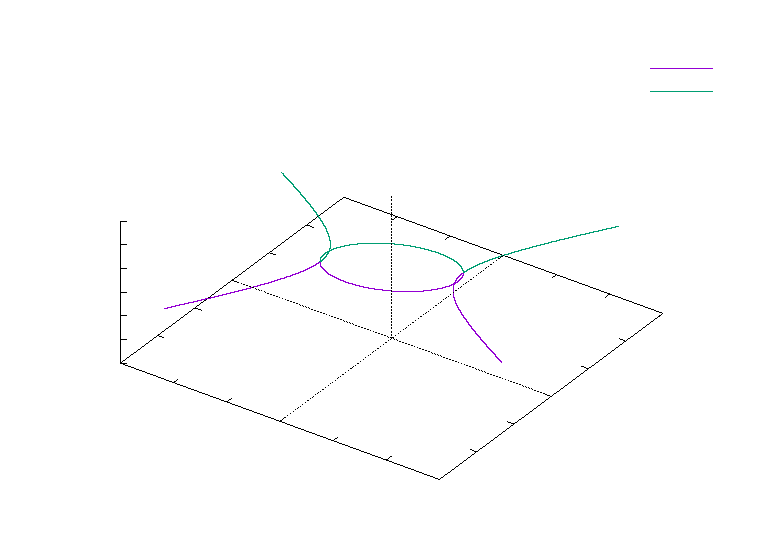
\includegraphics{plot}}%
    \gplfronttext
  \end{picture}%
\endgroup


\subsection*{b)} % Numbered section
%
\begin{align*}
x_{n+2}-ax_{x+1}+x_n=0\;\text{for}\;0\le a\le \infty\\
a=6 \implies x_{n+2}-6x_{x+1}+x_n=0\\
\text{Den karakteristiske ligningen er:}\\
r^2 - 6r + 1 = 0\\
r = \frac{6 \pm \sqrt{6^2 - 4}}{2}\\
r = 3 - 2\cdot \sqrt{2} \;\vee\; r = 3 + 2\cdot \sqrt{2}\\
x_n = \alpha \cdot \left( 3 - 2\cdot \sqrt{2} \right ) ^ n + \beta \cdot \left( 3 + 2\cdot \sqrt{2} \right ) ^ n\\
x_0 = \alpha + \beta\\
x_1 = \alpha \cdot \left( 3 - 2\cdot \sqrt{2} \right ) + \beta \cdot \left( 3 + 2\cdot \sqrt{2} \right )\\
\text{For at } x_n \text{ skal gå mot 0, må }\beta\text{ være 0. }\alpha \text{ kan være hva som helst.}\\
\text{Hva må } x_0,\; x_1 \text{ være for at } \beta \text{ er 0?}\\
\beta = \alpha - x_0\\
\beta = \frac{\alpha (3-2\sqrt{2}) - x_1}{3+2\sqrt{2}}\\
\text{For at } \beta \text{ skal være 0, må } x_0 = \alpha \text{ og } x_1 = -(2\sqrt{2}  - 3) \alpha
\end{align*}

\subsection*{c)}
\begin{align*}
	a&=0 \\
	x_{n+2}-0\cdot x_{n+1} + x_n &= 0\\
	r^2+1&=0\\
	r = -i \vee r &= i\\
	x_n &= \alpha \cdot \left(-i\right)^n + \beta \cdot i^n\\
	x_0 = 1 \implies \alpha \cdot \left(-i\right)^0 + \beta \cdot i^0 &= 1 \implies \alpha + \beta = 1\\
	x_1 = 1 \implies \alpha \cdot \left(-i\right)^1 + \beta \cdot i^1 &= 1 \implies -\alpha i + \beta i = 1\\
	\alpha &= 1 - \beta\\
	-\left(1 - \beta\right)i + \beta i &= 1\\
	-i + \beta i + \beta i &= 1\\
	2\beta i &= i+1\\
	\beta &= \frac{1+i}{2i}\\
	\beta &= \frac{1}{2} - \frac{1}{2} i\\
	\alpha &= 1 - \left(\frac{1}{2} - \frac{1}{2} i\right)\\
	\alpha &= \left(\frac{1}{2} + \frac{1}{2} i\right)\\
	x_n &=	\doubleunderline{\left(\frac{1}{2} + \frac{1}{2} i\right) \cdot (-i)^n + \left(\frac{1}{2} - \frac{1}{2} i\right) \cdot i^n}\\
\end{align*}
\subsection*{d)}
$i^n$ og $(-i)^n$ er periodisk med periode 4, siden $i^{4k}=1 \;\wedge\; (-i)^{4k}=1 \;\forall\; k \in \mathbb{Z}$. Resten av uttrykket er bare konstanter så $x_n$ sin periode vil være 4. Dersom $a=0$, vil uttrykket på være på formen $x_n = \alpha \cdot \left(-i\right)^n + \beta \cdot i^n$ hvor $\alpha$ og $\beta$ er konstanter. Perioden vil derfor alltid være 4 når $a=0$.
\subsection*{e)}
\begin{align*}
	a&= \sqrt{2}\\
	x_{n+2} - \sqrt{2}x_{n+1} + x_n &= 0\\
	r^2 - \sqrt{2}r + 1 &= 0\\
	r = \frac{1}{\sqrt{2}}-\frac{i}{\sqrt{2}} \;&\vee\; r =\frac{1}{\sqrt{2}}+\frac{i}{\sqrt{2}}\\
	x_n &= \alpha \cdot \left(\frac{1}{\sqrt{2}}-\frac{i}{\sqrt{2}}\right)^n + \beta \cdot \left(\frac{1}{\sqrt{2}}+\frac{i}{\sqrt{2}}\right)^n
\end{align*}

%------------------------------------------------
$x_n$ er periodisk med 4 som periode.
\section*{Oppgave 2}
\subsection*{a)}
\begin{align*}
	f(x)&= 2 \arctan (x) - \log(1+x^2),\; x \in \mathbb{R}\\
	f'(x)&= \frac{2}{1+x^2} - \frac{2x}{1+x^2}\\
	\text{Vi har lokale eksemalpunkter der f'(x) = 0}\\
	f'(x) = 0 \implies \frac{2}{1+x^2} - \frac{2x}{1+x^2} &= 0\\
	2 - 2x &= 0\\
	x &= 1\\
	f(1) = 2 \arctan (1) - \log(1 + 1^2) &= \frac{\pi}{2} - \log(2)\\
	\left(1,\;\frac{\pi}{2} - \log(2)\right) & \text{ er et lokalt ekstremalpunkt.}
\end{align*}
Vi bruker annenderiverttesten for å finne ut om det er et minimum- eller maksimumspunkt.
\begin{align*}
f''(x) &= \frac{2(x^2-2x-1)}{(1+x^2)^2}\\
f''(1) &= -1
\end{align*}
Siden $f''(1) < 0$, er $x=1$ et maksimumspunkt.
\subsection*{b)}
$f$ er konkav når $f''(x) < 0$ og konveks når $f''(x) > 0$.
Vi finner nullpunktene til $f''(x)$
\begin{align*}
	f''(x) &= 0\\
	\frac{2(x^2-2x-1)}{(1+x^2)^2} &= 0\\
	2(x^2-2x-1) &= 0\\
	x = 1 - \sqrt{2} \;&\vee\; x = 1 + \sqrt{2}\\
	f''(x) &= \frac{2(x-(1-\sqrt{2}))(x-(1+\sqrt{2}))}{{(1+x^2)^2}}
\end{align*}
\begin{tikzpicture}[%
negativ/.style={blue,dashed},
positiv/.style={red},
vertlinje/.style={dotted,opacity=.7},
node distance=1.5ex,
nullpunkt/.style={fill=white,inner sep= 1pt}]
\draw [->,>=stealth] (-5,0) node (linestart) {} -- (5,0) node (lineend) {};
\node (null1) at (-0.414,0) [label=above:$1-\sqrt{2}$] {};
\node (null2) at (2.414,0) [label=above:$1+\sqrt{2}$] {};
\node [matrix] (produktledd) [below left=of linestart]{
	\node [left] (f1) {$x-(1-\sqrt{2})$}; \\
	\node [left] (f2) {$x-(1+\sqrt{2})$}; \\
	\node [left] (f3) {$(1+x^2)^2$};\\
	\node [left] (f)  {$f''(x)$}; \\
};
\draw [vertlinje] (null1)       -- (null1 |- f);
\draw [vertlinje] (null2)       -- (null2 |- f);
\draw [positiv]   (null1 |- f1) -- (lineend |- f1);
\draw [negativ]   (f1)          -- (null1 |- f1) node[nullpunkt] {$0$};
\draw [negativ]   (null1 |- f)  -- (null2 |- f);
\draw [positiv]   (null2 |- f2) -- (lineend |- f2);
\draw [negativ]   (f2)          -- (null2 |- f2) node[nullpunkt] {$0$};
\draw [positiv]	  (f3)			-- (lineend |- f3);
\draw [positiv]   (f)           -- (null1 |- f)  node[nullpunkt] {$0$}
(null2 |- f) node[nullpunkt] {$0$} -- (lineend |- f);
\end{tikzpicture}

\noindent
$f$ er konkav på intervallet $\interval({1-\sqrt{2},\;1+\sqrt{2}})$ og konveks på intervallet $\interval({-\infty,\;1-\sqrt{2}}) \cup \interval({1+\sqrt{2},\;\infty})$

\section*{Oppgave 3}
\subsection*{a)}
\begin{align*}
	f(1) &= 1^2\ln{|1|^{1/2}} - 1^2 + \frac{1}{2} &= -\frac{1}{2}\\
	f(e^2) &= (e^2)^2 \ln{|e^2|^{1/2}} - (e^2)^2 + \frac{1}{2} &= \frac{1}{2}
\end{align*}
På grunn skjæringssetningen, og fordi $f$ er kontinuelig i $\interval[{1,\;e^2}]$, har $f$ et nullpunkt i intervallet.
\subsection*{b)}
\begin{align*}
	\lim_{x\to 0} f(x) &= \lim_{x\to 0} x^2\ln{(|x|^{1/2})} - x^2 + \frac{1}{2}\\
	&= \lim_{x\to 0} x^2\ln{(|x|^{1/2})} + \frac{1}{2}\\
	&= \lim_{x\to 0} \left(\frac{\ln{(|x|^{1/2})}}{1/x^2}\right) + \frac{1}{2}\\
&\neginfinf \quad \lim_{x\to 0} \left( \frac{\frac{1}{2x}}{-\frac{2}{x^3}} \right)+\frac{1}{2}\\
	&=\lim_{x\to 0} \left(-\frac{x^2}{4}\right) +\frac{1}{2}\\
	&= \frac{1}{2}
\end{align*}
Dersom vi definerer $f(0)=1/2$, er $f$ kontinuelig siden $\ln(x)$ er kontinuelig for alle x større enn 0 og $|x|^{1/2}$  aldri er negativ.

\subsection*{c)}

\begin{align*}
f'(0) &= \lim_{h\to 0}\frac{f(0 + h) - f(0)}{h}\\
&= \lim_{h\to 0} \frac{1/2 - 1/2}{h}\\
&= \lim_{h\to 0} \frac{0}{h}\\
&=\doubleunderline{0}
\end{align*}


\section*{Oppgave 4}
\subsection*{a)}
\begin{align*}
	\lim_{x\to +\infty} \frac{x^2-x+3}{x^3 - 2}\quad \infinf\quad \lim_{x\to +\infty} \frac{2x-1}{3x^2}
	\quad\infinf\quad \lim_{x\to +\infty} \frac{2}{6x}
	= 0
\end{align*}
\subsection*{b)}
\begin{align*}
	\lim_{x\to 1} \frac{x-1}{\sqrt{x+1} - \sqrt{2}} &= \lim_{x\to 1} \frac{(x-1)(\sqrt{x+1} + \sqrt{2})}{(\sqrt{x+1} - \sqrt{2})(\sqrt{x+1} + \sqrt{2})}\\
	&= \lim_{x\to 1} \frac{(x-1)(\sqrt{x+1} + \sqrt{2})}{x-1}\\
	&= \lim_{x\to 1} \sqrt{x+1} + \sqrt{2}\\
	&= 2\sqrt{2}
\end{align*}
\subsection*{c)}
\begin{align*}
	\lim_{x\to 0} \frac{\arctan(x^2)}{x\sin(x)} \;&\nillnill\; \lim_{x\to 0} \frac{\frac{2x}{x^4+1}}{\sin(x) + x\cos(x)}\\
	&\nillnill 	\lim_{x\to 0} \frac{\frac{2-6x^4}{(x^4+1)^2}}{2\cos(x) + x\sin(x)}\\
	&= \frac{2}{2} = 1
\end{align*}
%----------------------------------------------------------------------------------------
\section*{Oppgave 5}
Det er ingen oppgave 5 i oppgavesettet
\section*{Oppgave 6}
\subsection*{a)}
Løsningene til ligningen $e^{x/2} = 2-2x$ er det samme som nullpunktene til funksjonen $f(x) = e^{x/2} - 2+2x$
\begin{align*}
	f(0) = e^{0/2} - 2 + 2\cdot 0 &= -1\\
	f(1) = e^{1/2} - 2 + 2 \cdot 1 &= e^{1/2}
\end{align*}
Siden $f$ er kontinuelig på $\interval[{0,\;1}]$ og to punkter i intervallet har forskjellig fortegn, har $f$ minst ett nullpunkt i intervallet.
\subsection*{b)}
$f$ er strengt voksende $$f'(x) = \frac{1}{2} e^{x/2} + 2$$
$f$ har derfor bare ett nullpunkt i $\interval({-\infty,\;\infty})$.
\subsection*{c)}
\begin{align*}
	x_{n+1} &= x_n - \frac{f(x_n)}{f'(x_n)}\\
	x_1 &= x_0 - \frac{f(x_0)}{f'(x_0)}\\
	x_0 &= 0\\
	f(0) &= -1\\
	f'(0) &= \frac{1}{2} e^{0/2} + 2 = \frac{5}{2}\\
	x_1 &= x_0 - \frac{f(x_0)}{f'(x_0)}\\
	x_1 &= 0 - \frac{-1}{\frac{5}{2}} = \frac{2}{5}
\end{align*}
$f''(x) = \frac{1}{4} e^{x/2}$
\skippingparagraph
Newtons metode finner neste iterasjon ved å ta nullpunktet til tangenten i $x_n$. Siden $f''(x)$ alltid er positiv vil dette nullpunkt alltid være for stort når $f(x) < 0$. Siden $f(0) < 0$, er løsningen på ligningen mindre enn $\frac{5}{2}$.
\section*{Oppgave 7}
\subsection*{a)}
\begin{align*}
	z^2 - 2\cos(\theta) z + 1 &= 0\\
	z &= \frac{2\cos \theta \pm \sqrt{4 \cos^2\theta - 4}}{2}\\
	 &= \frac{2 \cos \theta \pm \sqrt{4}\sqrt{\cos^2\theta - 1}}{2}\\
	&= \cos \theta \pm \sqrt{\cos^2 \theta - 1}\\
	&= \cos\theta\pm\sqrt{-\sin^2\theta}\tag{$\cos^2\theta - 1 = -\sin^2 \theta$}\\
	&= \cos\theta\pm\sqrt{-1}\sqrt{\sin^2\theta}\\
	&= \cos \theta \pm i\sin\theta\\
	e^{i\theta} &= \cos\theta + i\sin\theta\\
	e^{-i\theta} &= \cos\theta - i\sin\theta\\
	z = e^{i\theta} &\vee z = e^{-i\theta}
\end{align*}
\subsection*{b)}
\begin{align*}
	\theta&=\frac{\pi}{6}\\
	z_1 &= \cos\frac{\pi}{6} + i\sin\frac{\pi}{6} = \frac{\sqrt{3}}{2} + \frac{i}{2}\\
	z_2 &= \cos\frac{\pi}{6} - i\sin\frac{\pi}{6} = \frac{\sqrt{3}}{2} - \frac{i}{2}
\end{align*}
\begin{figure}[H]
\centering
\begin{tikzpicture}
\begin{axis}[
axis lines=middle,
xmin=-0.5, xmax=1.5,
ymin=-1, ymax=1,
xlabel=$x$,
ylabel=$y$]
\addplot[color=red,only marks, mark=x, thick] coordinates {
	(0.86602,0.5)
	(0.86602,-0.5)
};
\end{axis}
\end{tikzpicture}
\end{figure}
\begin{align*}
	z_1^2 + z_2^2 &= \left(e^{i\pi/6}\right)^2 + \left(e^{-i\pi/6}\right)^2\\
	&=e^{i\pi/3}+e^{-i\pi/3}\\
	&=\cos\frac{\pi}{3}+i\sin\frac{\pi}{3}+\cos\frac{\pi}{3}-i\sin\frac{\pi}{3}\\
	&=\frac{1}{2} + \frac{1}{2} = 1
\end{align*}

\section*{Oppgave 8}
\subsection*{a)}

En funksjon er injektiv dersom den er strengt voksende.
$$f'(x) = e^{\left(x^3\right)} \cdot 3x^2$$
$e^{\left(x^3\right)}$ og $3x^2$ er positivt for alle x i $\interval({0,\; \infty})$ så $f$ er strengt voksende og injektiv.
\skippingparagraph
$f$ er surjektiv dersom for enhver $y$, finnes det en $x$ slik at $y=f(x)$.
\begin{align*}
	y&=e^{\left(x^3\right)}\\
	\sqrt[3]{y}&=\sqrt[3]{e^{\left(x^3\right)}} = e^x\\
	\ln\left(\sqrt[3]{y}\right) &= \ln(e^x) = x\\
	f^{-1}(x) &= \ln\left(\sqrt[3]{x}\right)
\end{align*}
\noindent
For enhver $y$ finnes det en $x$ slik at $y=f(x)$. Denne $x$ er $\ln\left(\sqrt[3]{y}\right)$. $f$ er således surjektiv.
\subsection*{b)}
Vi fant $f^{-1}(x)$ i a).
$$f^{-1}(x) = \ln\left(\sqrt[3]{x}\right)$$
\section*{Oppgave 9}
\subsection*{a)}
$x^2$ og $\arctan(x)$ er kontinuelige på $\interval({-\infty,\;\infty})$, så $f$ er også det.
$$f'(x) = 2x\arctan x + x^2\frac{1}{1+x^2}=x\left(\arctan x + \frac{x}{1+x^2}\right)$$

\begin{tikzpicture}[%
negativ/.style={blue,dashed},
positiv/.style={red},
vertlinje/.style={dotted,opacity=.7},
node distance=1.5ex,
nullpunkt/.style={fill=white,inner sep= 1pt}]
\draw [->,>=stealth] (-5,0) node (linestart) {} -- (5,0) node (lineend) {};
\node (null1) at (0,0) [label=above:$0$] {};
\node [matrix] (produktledd) [below left=of linestart]{
	\node [left] (f1) {$x$}; \\
	\node [left] (f2) {$\arctan x+\frac{x}{1+x^2}$};\\
	\node [left] (f)  {$f'(x)$}; \\
};
\draw [vertlinje] (null1)       -- (null1 |- f);
\draw [positiv]   (null1 |- f1) -- (lineend |- f1);
\draw [negativ]   (f1)          -- (null1 |- f1) node[nullpunkt] {$0$};
\draw [negativ]   (null1 |- f)  -- (null2 |- f);
\draw [positiv]   (null1 |- f2) -- (lineend |- f2);
\draw [negativ]   (f2)          -- (null1 |- f2) node[nullpunkt] {$0$};
\draw [positiv]   (null1 |- f)  -- (lineend |- f);
\draw [positiv]   (f)           -- (null1 |- f) node[nullpunkt] {$0$};

\end{tikzpicture}

$f'(x) \ge 0 \;\forall\; x \in \interval({-\infty,\;\infty}) \implies f \text{ er injektiv}$

\subsection*{b)}
\subsection*{c)}

$$f'(1) = 2\cdot1\cdot \arctan(1) + 1^2 \cdot \frac{1}{1+1^2}=\frac{\pi+1}{2}$$
\begin{align*}
	y-y_1 &= a(x-x_1)\\
	&y = \left(\frac{\pi+1}{2}\right) (x-1) + \frac{\pi}{4}\\
	=&y= \left(\frac{\pi+1}{2}\right) x - \left(\frac{\pi+1}{2}\right) + \frac{\pi}{4}\\
	=&\doubleunderline{y= \left(\frac{\pi+1}{2}\right) x - \frac{3\pi+2}{4}}
\end{align*}
Tangent til $y=f^{-1}(x)$ i $(\pi/4,\;1)$
\begin{align*}
\frac{d f^{-1}}{dx} (x) &= \frac{1}{f'(f^{-1}(x))}\\
\frac{d f^{-1}}{dx} \left(\frac{\pi}{4}\right) &= \frac{1}{f'(f^{-1}(\frac{\pi}{4}))}\\
&= \frac{1}{f'(1)} = \frac{1}{\frac{\pi+1}{2}}= \frac{2}{\pi+1}
\end{align*}

Vi finner ligningen til tangenten

\begin{align*}
		y-y_1 = a(x-x_1) &= y - 1 = \left(\frac{2}{\pi+1}\right)\left(x-\frac{\pi}{4}\right)\\
		&= y = \left(\frac{2}{\pi+1}\right) x - \left(\frac{2}{\pi+1}\right) \left(\frac{\pi}{4}\right) + 1\\
		&= \doubleunderline{y = \left(\frac{2}{\pi+1}\right) x - \frac{\pi}{2(1+\pi)} + 1}
\end{align*}

\subsection*{d)}
\begin{align*}
	f''(x) = 2 \arctan x + 2x \frac{1}{1+x^2} + x^2 \cdot \left(-\frac{2x}{(1+x^2)^2}\right)
\end{align*}
Alle ledd er positive når $x>0$ og negative når $x<0$. $f$ er derfor konkav på $\interval({-\infty,\;0})$ og konveks på $\interval({0,\;\infty})$
\section*{Oppgave 10}
\subsection*{a)}
\begin{align*}
	A(r+\Delta r)&\approx A(r) + A'(r)\cdot \Delta r\\
	A'(r) &= \pi \sqrt{r^2+h^2} + \pi 2r^2 \cdot \frac{1}{2\sqrt{r^2 + h^2}} \\
	&= \pi\left(\sqrt{r^2+h^2} + \frac{r^2}{\sqrt{r^2+h^2}}\right)\\
	&= \pi\left( \frac{r^2+h^2}{\sqrt{r^2+h^2}} + \frac{r^2}{\sqrt{r^2+h^2}} \right)\\
	&= \frac{\pi (2r^2 + h^2)}{\sqrt{r^2+h^2}}\\
	A(r+\Delta r) &\approx \pi r \sqrt{r^2+h^2} + \frac{\pi (2r^2 + h^2)}{\sqrt{r^2+h^2}} \Delta r
\end{align*}
\subsection*{b)}

Ved middelverdisetningen vet vi at det finnes et punkt $c$, slik at
\begin{align*}
f'(c)&=\frac{f(b) - f(a)}{b - a}\\
&= \frac{f(a+h) - f(a)}{\slashed{a} + h - \slashed{a}}\tag{$a+h = b$}\\
&= \frac{f(a) + f'(a)h + \eta(h)h - f(a)}{h}\tag{$f(a+h) = f(a) + f'(a)h + \eta(h)h$}\\
&= \frac{f'(a)h + \eta(h)h}{h}\\
&= f'(a) + \eta(h)
\end{align*}
Dersom vi flytter om på leddene finner vi:
$$f'(c) = f'(a) + \eta(h) \iff \eta(h) = f'(c) - f'(a)$$
\end{document}

